\documentclass{beamer}
\usepackage{pgfpages}
\usepackage[backend=bibtex]{biblatex}
\usepackage{multicol}
\usepackage{multimedia}
\usepackage[absolute,overlay]{textpos}
\usepackage{parskip}
\usepackage{hyperref}
\usepackage{lmodern}
\usepackage{bbding}
\usepackage[absolute,overlay]{textpos}
\usepackage{framed} %Used to shade important equations, color devined with shadecolor
\hypersetup{colorlinks=true, urlcolor=blue}
\setlength{\parskip}{\smallskipamount}
\colorlet{shadecolor}{cyan}
%\usepackage[texcoord,grid,gridunit=mm,gridcolor=red!10,subgridcolor=green!10]{eso-pic} %DELETE when done with grid
\setbeameroption{hide notes} % Only slides
%\setbeameroption{show only notes} % Only notes
%\setbeameroption{show notes on second screen=right} % Both
%\bibliography{../../papers/references.bib}
\setbeamerfont{footnote}{size=\tiny}
%\AtEveryCitekey{\clearfield{title}}

%
% Choose how your presentation looks.
%
% For more themes, color themes and font themes, see:
% http://deic.uab.es/~iblanes/beamer_gallery/index_by_theme.html
%
\mode<presentation>
{
\usetheme{Warsaw}      % or try Darmstadt, Madrid, Warsaw, ...
\usecolortheme{default} % or try albatross, beaver, crane, ...
\usefonttheme{default}  % or try serif, structurebold, ...
\setbeamertemplate{navigation symbols}{}
\setbeamertemplate{caption}[numbered]
} 

\usepackage[english]{babel}
%\usepackage[utf8x]{inputenc} %Doesn't play well with biblatex
\usepackage{amssymb}
\usepackage{bm}
\usepackage{color}
\usepackage{graphicx}
\setbeamercovered{invisible}
\setbeamercovered{%
again covered={\opaqueness<1->{100}}} %This changes the opaqueness of each bullet

\newcommand{\red}[1]{{\color{red}{#1}}}
\newcommand{\checkH}[2]{\begin{textblock*}{1cm}(#1,#2){\Huge \red{\Checkmark}}\end{textblock*}}
\newcommand{\checkh}[2]{\begin{textblock*}{1cm}(#1,#2){\huge \red{\Checkmark}}\end{textblock*}}
\newcommand{\checkL}[2]{\begin{textblock*}{1cm}(#1,#2){\Large \red{\Checkmark}}\end{textblock*}}
\newcommand{\checkl}[2]{\begin{textblock*}{1cm}(#1,#2){\large \red{\Checkmark}}\end{textblock*}}
\renewcommand{\rm}[1]{\mathrm{#1}}

\title[{\color{white}{Chapters 2.5-7}}]{Physics 121: \\ Free Fall, Inclined Plane Motion}
\author{Cody Petrie}
\institute{Mesa Community College}
\date{}

\begin{document}

%\setbeamertemplate{frametitle}[default][center]
\begin{frame}
\titlepage
\end{frame}

% Uncomment these lines for an automatically generated outline.
%\begin{frame}{Outline}
%  \tableofcontents
%\end{frame}

% Commands to include a figure:
%\begin{figure}
%\includegraphics[width=\textwidth]{your-figure's-file-name}
%\caption{\label{fig:your-figure}Caption goes here.}
%\end{figure}

\begin{frame}{Reminders}
\begin{itemize}
   \item There is a HW assignment due this Thursday on Mastering Physics. How did last week go?
   \item On Thursday we are doing the V: Vectors lab. This is in the appendix of the labs so make sure to bring it (just in case some of you only bring 2-3 labs at a time like me).
\end{itemize}
\end{frame}

\begin{frame}{Quick Review - Derivatives}
\begin{itemize}
   \item<1-> $v_s = \lim\limits_{\Delta t \rightarrow 0} \frac{\Delta s}{\Delta t} = \frac{ds}{dt}$ ~~~(Instantaneous Velocity)
   \item<2-> $\frac{d}{dt} ct^n = nct^{n-1}$
   \item<3-> The instantaneous velocity is the slope of the tangent line to the $x(t)$ curve.
\end{itemize}
\uncover<3>{
\begin{center}
   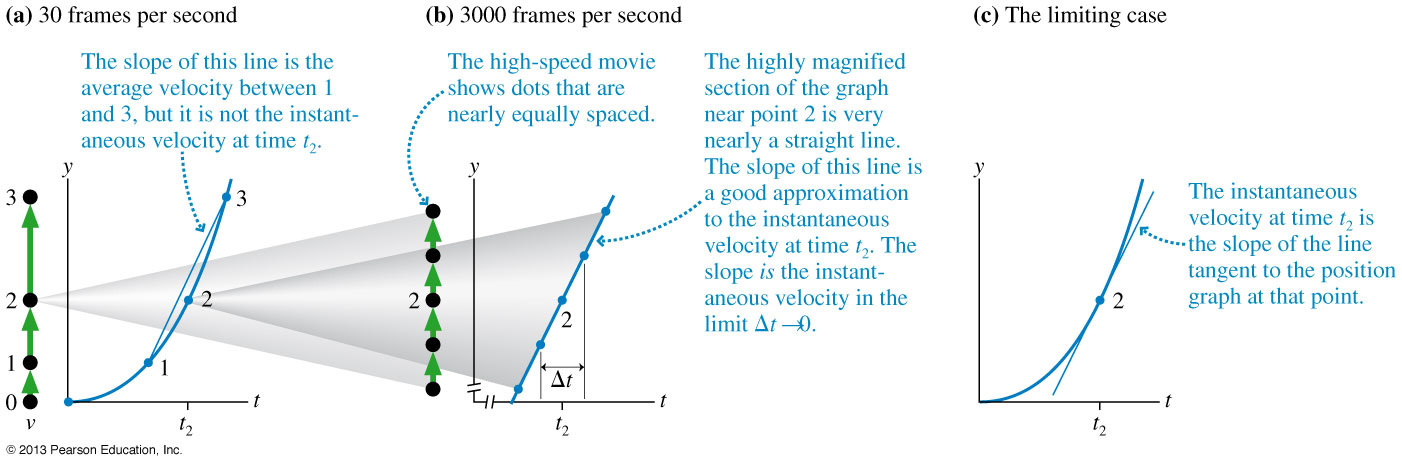
\includegraphics[width=\textwidth]{../figures/02_09_Figure.jpg}
\end{center}}
\end{frame}

\begin{frame}{Quick Review - Integrals}
\begin{itemize}
   \item<1-> If you want to determine the position at time $t$ given the position at time $t=0$ and the velocity you use an integral.
   \begin{equation*}
      s_f = s_i + \lim\limits_{\Delta t \rightarrow 0} \sum\limits_{k=1}^N (v_s)_k\Delta t = s_i + \int\limits_{t_i}^{t_f}v_s dt
   \end{equation*}
   \uncover<2>{
   \begin{equation*}
      \int\limits_{t_i}^{t_f} ct^ndt = \uncover<2>{\frac{ct^{n+1}}{n+1}\bigg|_{t_i}^{t_f} = \frac{ct_f^{n+1}}{n+1} - \frac{ct_i^{n+1}}{n+1} ~~~~~ (n \ne -1)}
   \end{equation*}}
   \item<3-> This is the area under the $v(t)$ curve.
\end{itemize}
\uncover<3>{
\begin{center}
   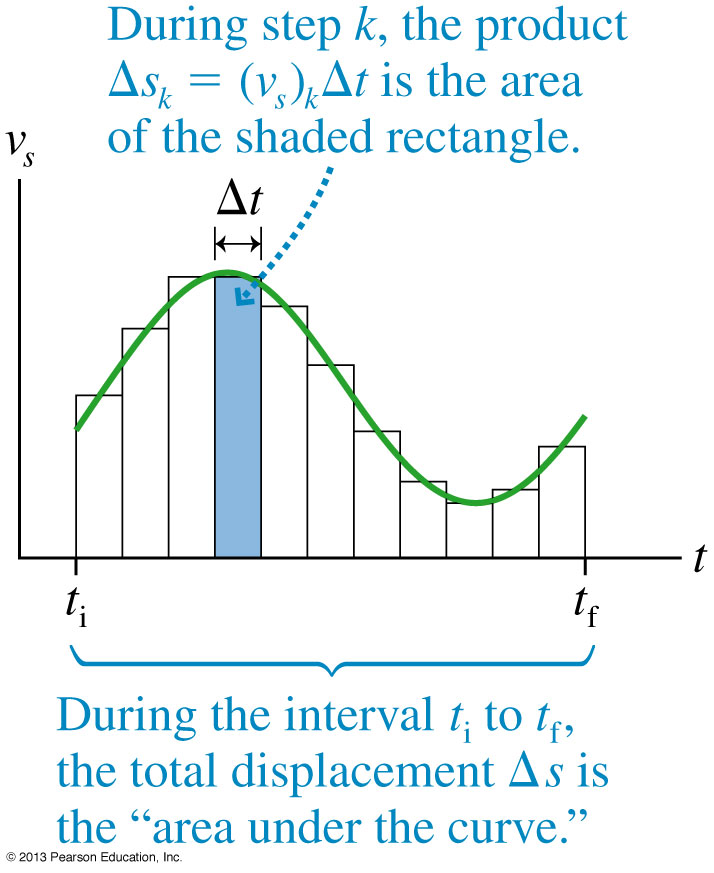
\includegraphics[width=0.25\textwidth]{../figures/02_16_Figure.jpg}
\end{center}}
\end{frame}

\begin{frame}{Quick Review - Acceleration}
\begin{itemize}
   \item<1-> The acceleration of an object is how much an object changes it's velocity in a given amount of time, (m/s)/s $\rightarrow$ m/s$^2$.
   \item<2->The average acceleration is given by the slope of the $v(t)$ curve.
   \uncover<2>{
   \begin{equation*}
      a_{ave} = \frac{\Delta v}{\Delta t}
   \end{equation*}}
   \item<3-> Using these ideas you can write down the kinematic equations (which will be used A LOT in this class to calculation the motion of objects in various situations with constant acceleration)
\end{itemize}
\uncover<3->{
\begin{align*}
   v_f &= v_i + a\Delta t \\
   s_f &= s_i + v_i\Delta t + \frac{1}{2}a(\Delta t)^2 \\
   v_f^2 &= v_i^2 + 2a\Delta s
\end{align*}}
\end{frame}

\begin{frame}{Free Fall}
\begin{center}
   \color{blue}{\Huge FREE FALL MOTION!}
\end{center}
\end{frame}

\begin{frame}{Free Fall}
\begin{itemize}
   \item Galileo Galilei (1564-1642) supposedly dropped objects from bell towers in Italy to study object in free fall motion. Here are two of his main discoveries.
   \begin{columns}
   \begin{column}{0.5\textwidth}
   \begin{center}
      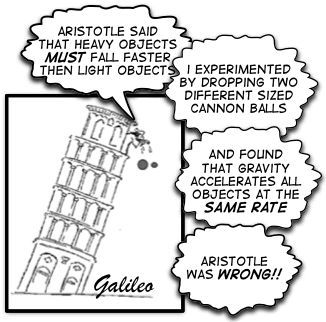
\includegraphics[width=\textwidth]{../figures/galileo_tower.jpg}
   \end{center}
   \end{column}
   \begin{column}{0.5\textwidth}
   \begin{enumerate}
      \item If you drop two objects from the same height, if there is no air resistance, will hit the ground at the same time at the same speed.
      \item Any two objects in free fall, regardless of their mass, have the same acceleration, $\vec{a}_{\text{free fall}}$.
   \end{enumerate}
   \uncover<2>{\red{What about a feather and a bowling ball?}}
   \end{column}
   \end{columns}
\end{itemize}
\end{frame}

\begin{frame}{Feather vs. Bowling Ball Video}
\begin{center}
   \Huge \href{https://www.youtube.com/watch?v=E43-CfukEgs}{Vacuum Chamber}
\end{center}
\end{frame}

\begin{frame}{Free Fall}
\begin{itemize}
   \item The rate at which things fall close to the surface of the earth (average at sea level) is
   \begin{equation*}
      \vec{a}_{\text{free fall}} = (9.80 \text{m/s}^2, \text{vertically downward})
   \end{equation*}
   \item<2-> Vertically downward means toward the center of the earth (this is because the acceleration is due to gravity).
   \item<3-> The magnitude of this acceleration is $g=9.80$ m/s$^2$.
   \begin{itemize}
      \item<3-> As a result $g$ is always a positive number, so $\vec{a} = -g\hat{y}$.
   \end{itemize}
   \item<4-> Since free fall motion is {\it constant acceleration} motion you can use the equations mentioned before, but with $a=-g$.
   \item<5-> $g=9.80$ m/s$^2$ only on earth. We'll see more about this when we talk about gravity.
\end{itemize}
\end{frame}

\begin{frame}{Quick Check}
\begin{center}
   A ball is tossed straight up in the air. At its very highest point, the ball's instantaneous acceleration $a_y$ is
\end{center}
\begin{enumerate}[A.]
   \item Positive
   \item Negative
   \item Zero
\end{enumerate}
\only<2->{\checkL{0.7cm}{4.6cm}}
\end{frame}

\begin{frame}{Quick Check}
\begin{center}
   \only<1>{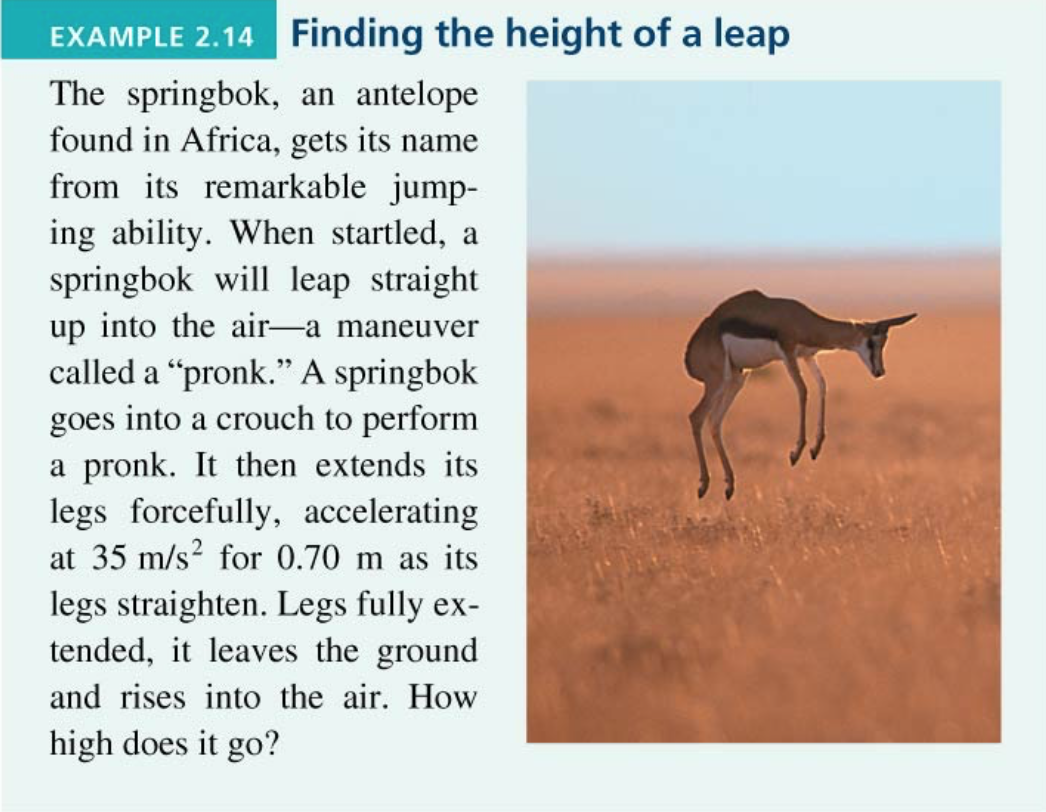
\includegraphics[width=\textwidth]{../figures/Ex2_14.png}}
   \only<2>{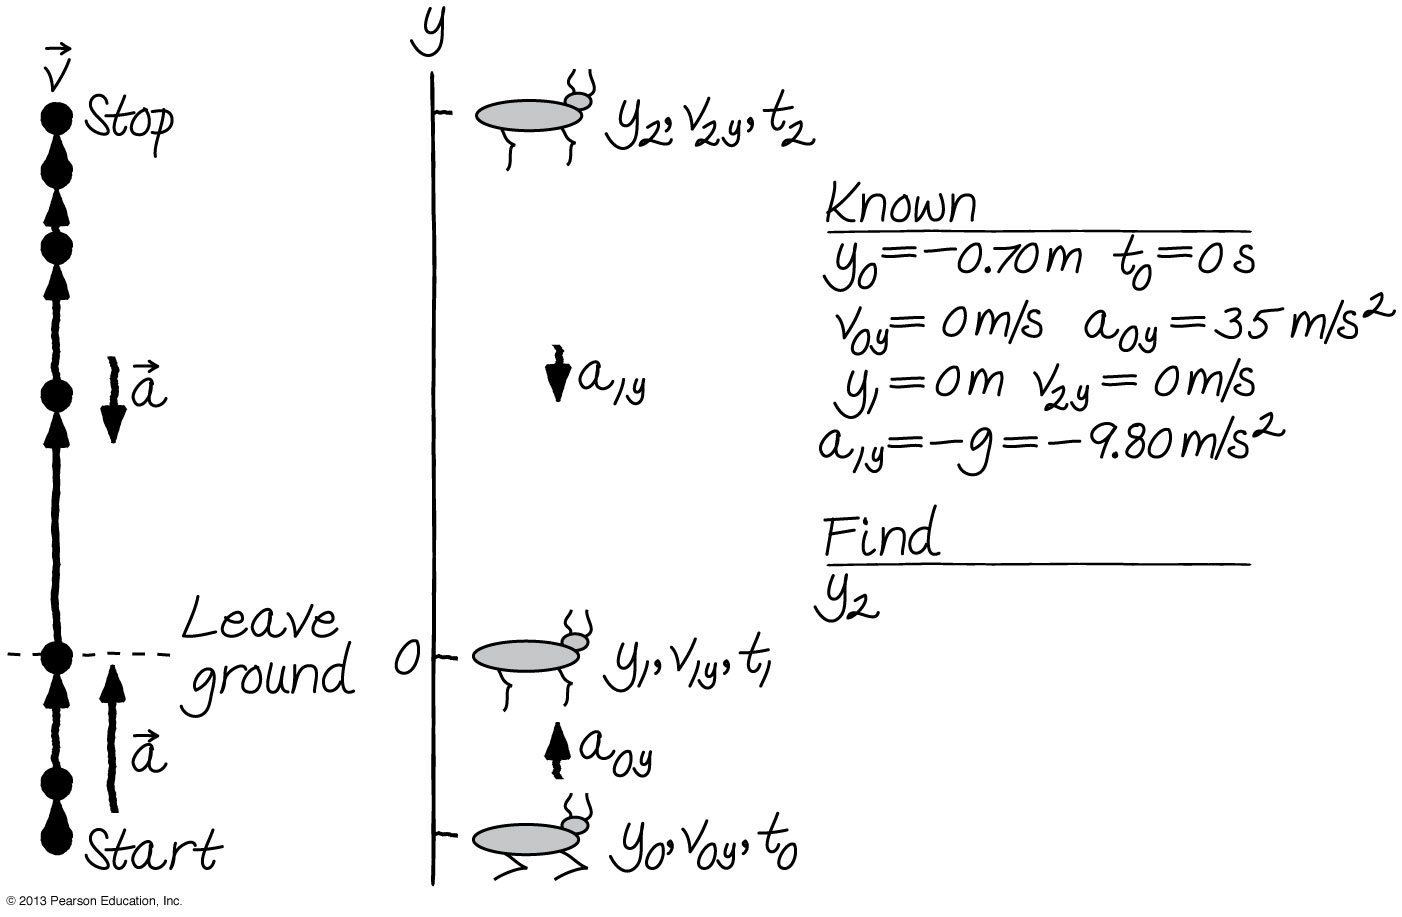
\includegraphics[width=\textwidth]{../figures/02_30_Figure.jpg}}
   \only<3->{
   \begin{itemize}
      \item First find the velocity at the end of the ``push up" time period. We know position but not time so which kinematic equation should be use?\\ \uncover<4>{$v_{1y}^2 = v_{0y} + 2a_{0y}\Delta y$} \uncover<5>{$\rightarrow v_{1y} = 7.0$ m/s}
      \item<6-> Now solve for the final height. What equation(s) would you use? Think about what you know and don't know.
      \begin{itemize}
         \item<7-> Use $v_f = v_i + a\Delta t$ to solve for $\Delta t$ and then $s_f = s_i + v_i\Delta t + \frac{1}{2}a(\Delta t)^2$ to solve for $y_2$. OR use one equaiton, $v_f^2 = v_i^2 + 2a\Delta s$ alone. \uncover<8>{$\rightarrow y_2 = 2.5$ m.}
      \end{itemize}
   \end{itemize}
   }
\end{center}
\end{frame}

\begin{frame}{Inclined Plane}
\begin{center}
   \color{blue}{\Huge Motion on an Inclined Plane}
\end{center}
\end{frame}

\begin{frame}{Inclined Plane}
%\begin{columns}
%\begin{column}{0.5\textwidth}
%   \begin{center}
%      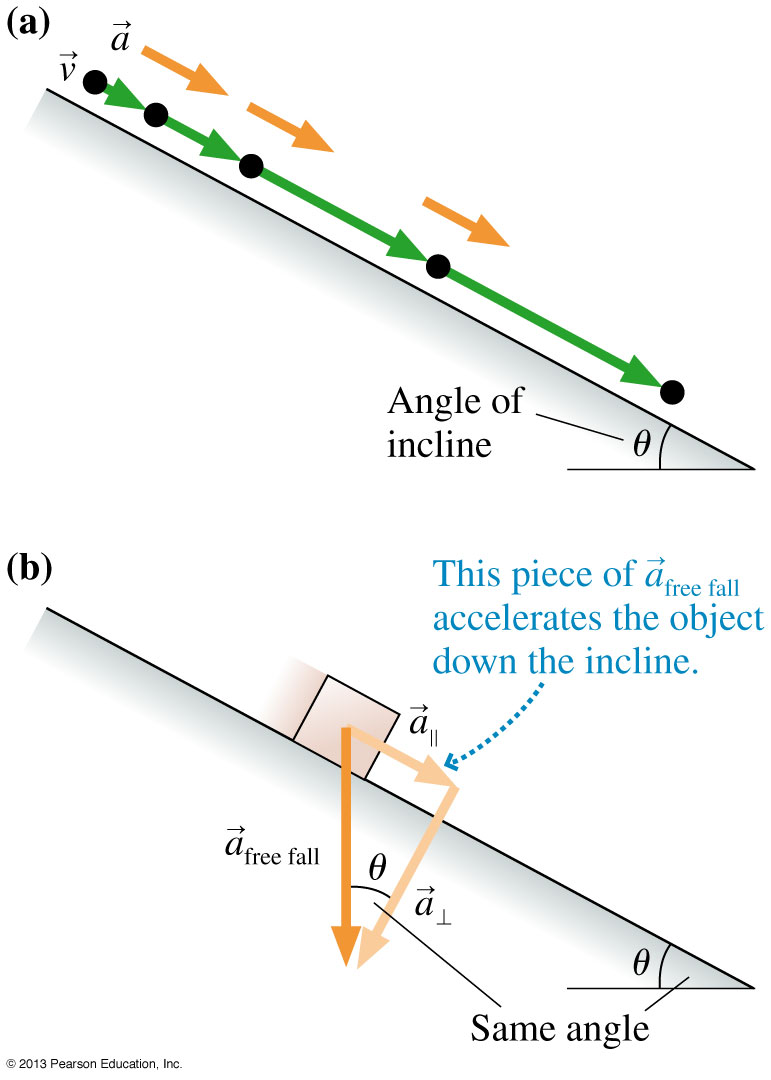
\includegraphics[height=\textheight]{../figures/02_31_Figure.jpg}
%   \end{center}
%\end{column}
%\begin{column}{0.5\textwidth}
%\begin{itemize}
%   \item What is different between free fall motion and motion on an inclines plane (i.e. ball rolling down a ramp)?
%   \begin{itemize}
%      \item<2-> $\vec{a}$ changes and the direction of the motion is down the ramp.
%   \end{itemize}
%\end{itemize}
%\end{column}
%\begin{columns}
\begin{columns}
\begin{column}{0.5\textwidth}
\begin{itemize}
   \item What is different between free fall motion and motion on an inclines plane (i.e. ball rolling down a ramp)?
   \begin{itemize}
      \item<2-> $\vec{a}$ changes and the direction of the motion is down the ramp.
   \end{itemize}
   \item<2-> The vector $\vec{a}_{ff}$ can be broken into two components, $\vec{a}_\bot$ and $\vec{a}_\parallel$
   \item<3-> Somehow the surface blocks $\vec{a}_\bot$ (which we'll talk about later), which means that the acceleration alone the surface is given by
   \uncover<3>{\begin{equation*}
      a_s = a_\parallel = \pm g\sin{\theta}
   \end{equation*}}
\end{itemize}
\end{column}
\begin{column}{0.5\textwidth}
\uncover<2>{
\begin{center}
   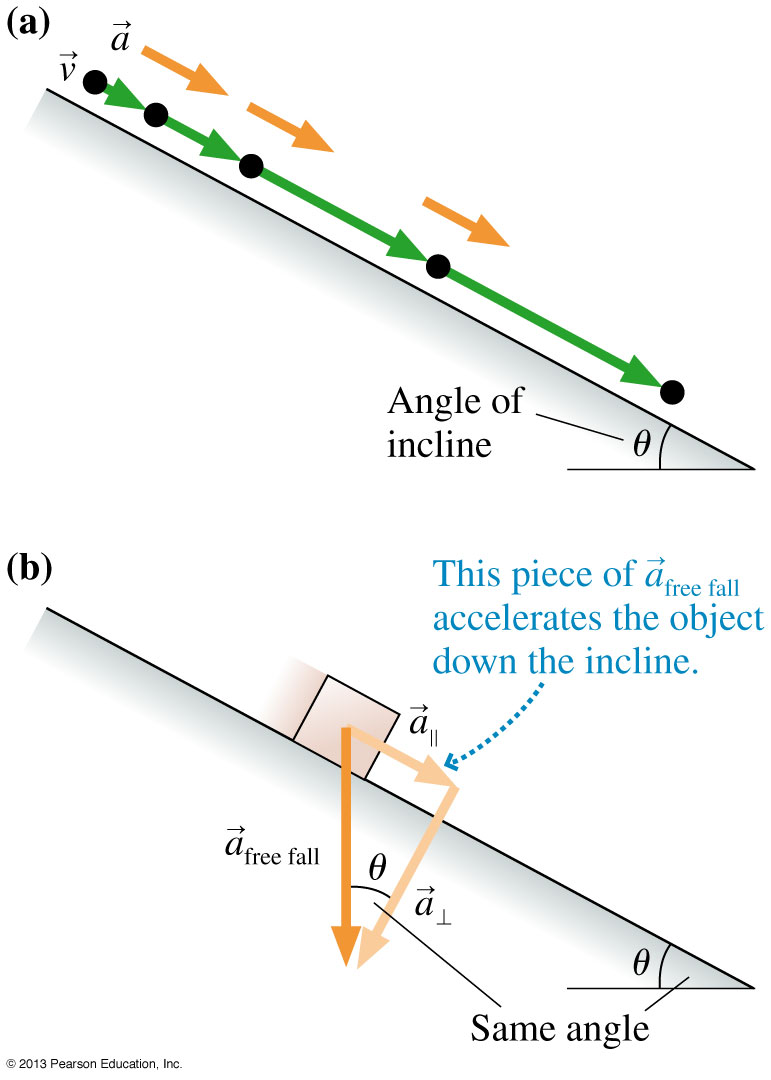
\includegraphics[height=0.8\textheight]{../figures/02_31_Figure.jpg}
\end{center}}
\end{column}
\end{columns}
\end{frame}

\begin{frame}{Quick Check}
\begin{center}
   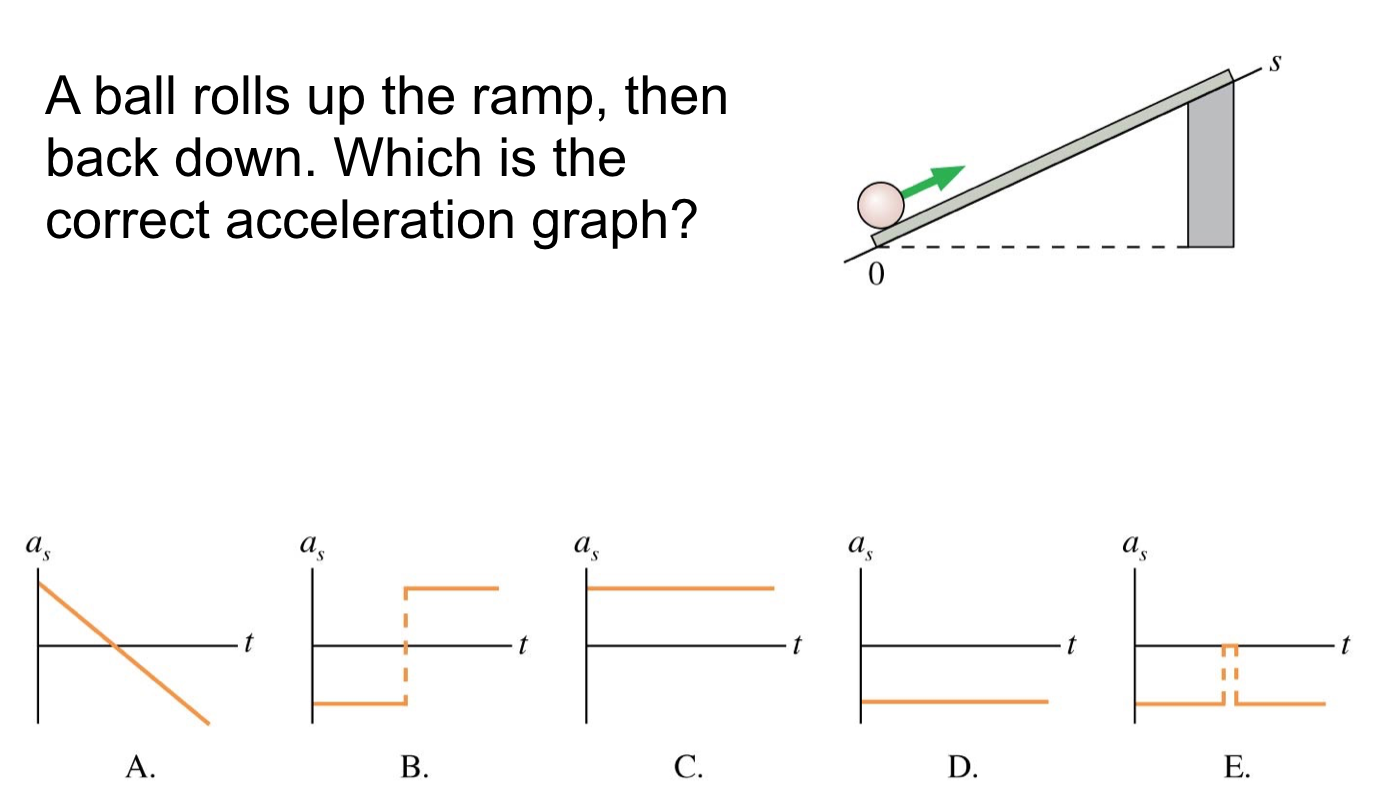
\includegraphics[width=\textwidth]{../figures/QC2_19.png}
\end{center}
\only<2->{\checkL{8.5cm}{7.6cm}}
\end{frame}

\begin{frame}{Quick Check}
\begin{center}
   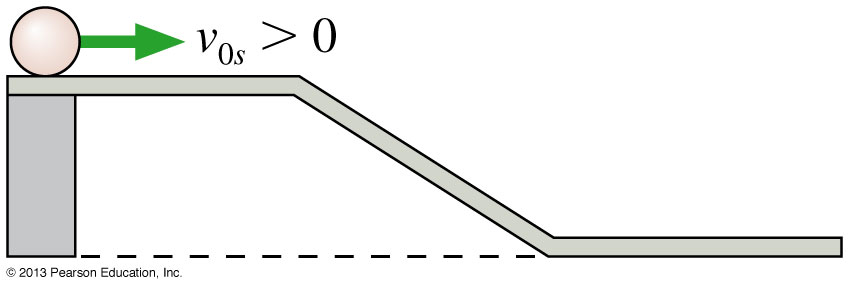
\includegraphics[width=0.6\textwidth]{../figures/02_35_Figure.jpg}
\end{center}
\begin{columns}
\begin{column}{0.5\textwidth}
\begin{center}
   Draw the $x$, $v_s$ and $a_s$ vs. $t$ graphs for a ball rolling down the inclined plane here. Include all three sections of motion.
\end{center}
\end{column}
\begin{column}{0.5\textwidth}
   \uncover<2>{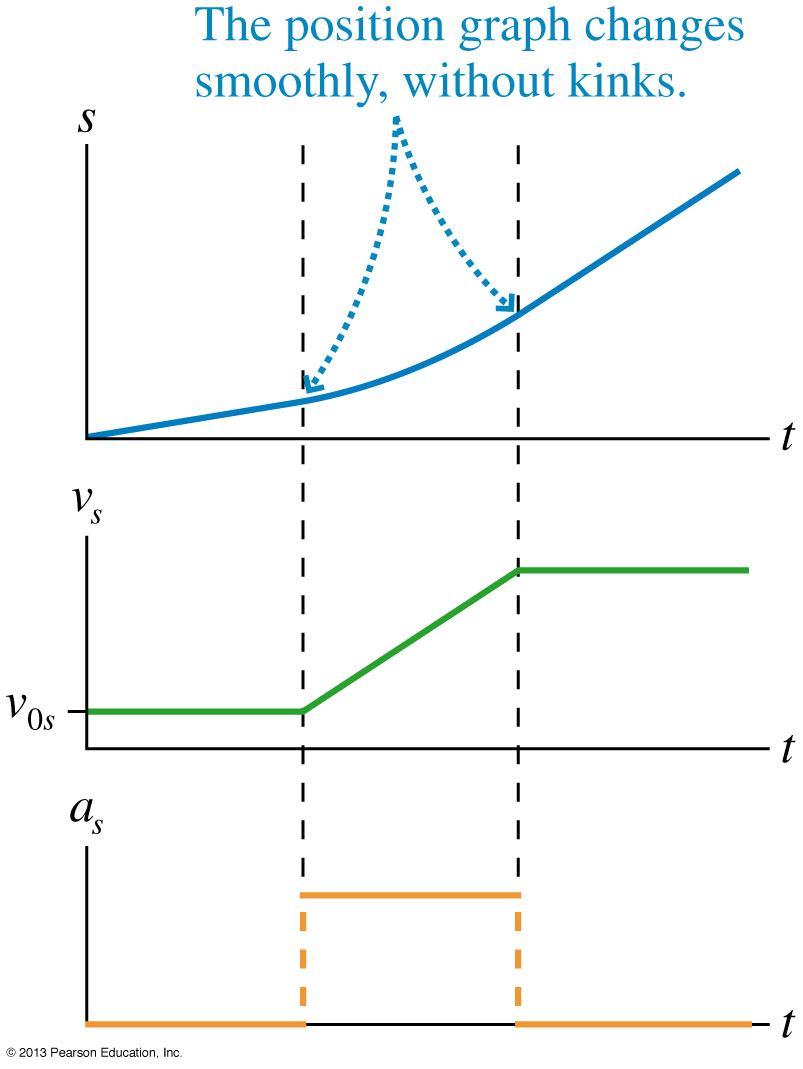
\includegraphics[height=0.65\textheight]{../figures/02_36_Figure.jpg}}
\end{column}
\end{columns}
\end{frame}

\begin{frame}{Instantaneous Acceleration}
\begin{center}
   \color{blue}{\Huge Instantaneous Acceleration}
\end{center}
\end{frame}

\begin{frame}{Instantaneous Acceleration}
\begin{columns}
\begin{column}{0.7\textwidth}
\begin{center}
   Realistic motion often doesn't have constant acceleration. Here is the realistic motion of a car pulling away from a stop sign.
\end{center}
\end{column}
\begin{column}{0.3\textwidth}
   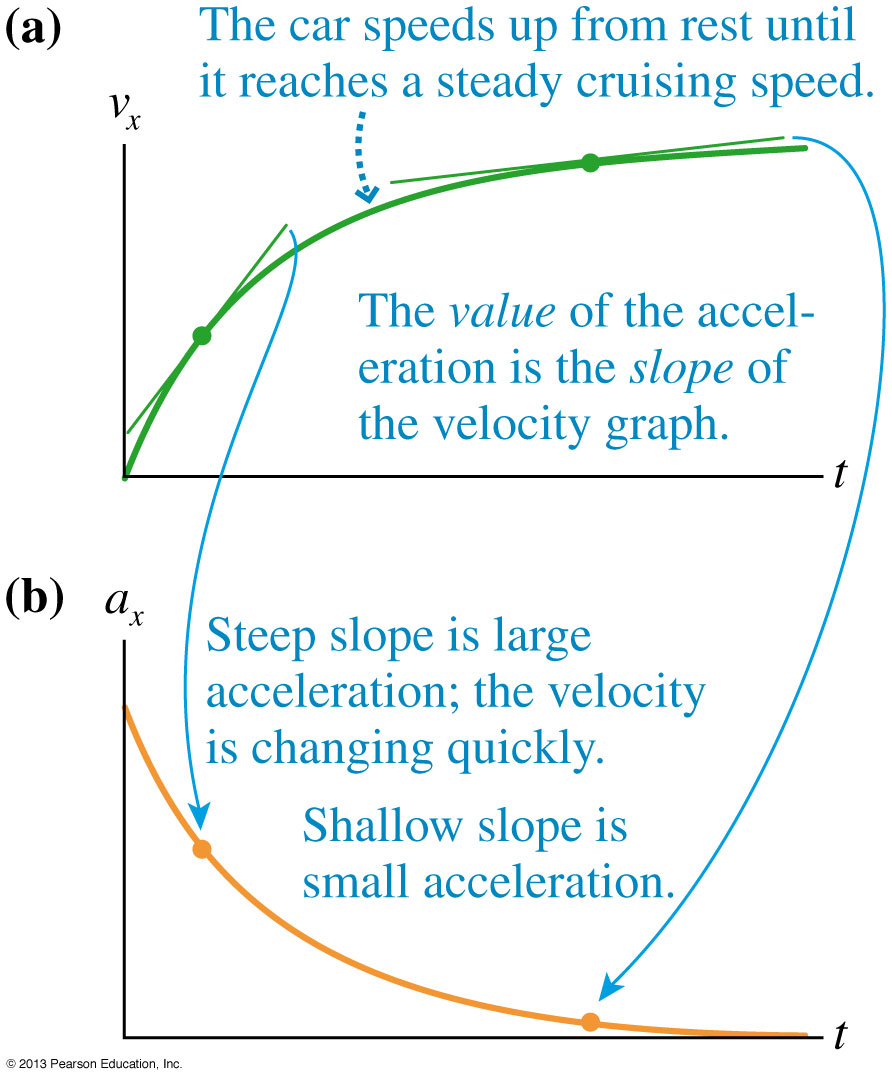
\includegraphics[width=\textwidth]{../figures/02_39_Figure.jpg}
\end{column}
\end{columns}
\begin{itemize}
   \item<2-> Just like we did with instantaneous velocity we can write the instantaneous acceleration as a derivative of the velocity. \\ \begin{center}$a_s = \frac{dv_s}{dt}$\end{center}
   \item<3-> Also you can use an integral determine $v(t)$ from the acceleration and initial $v(t=0)$ \\ \begin{center}$v_{fs} = v_{is} + \int\limits_{t_i}^{t_f} a_s dt$\end{center}
\end{itemize}
\end{frame}

\begin{frame}{Instantaneous Acceleration}
\begin{center}
   If an object is initially moving at 10 m/s and has this acceleration curve what is the velocity of the object at t=8 s?
   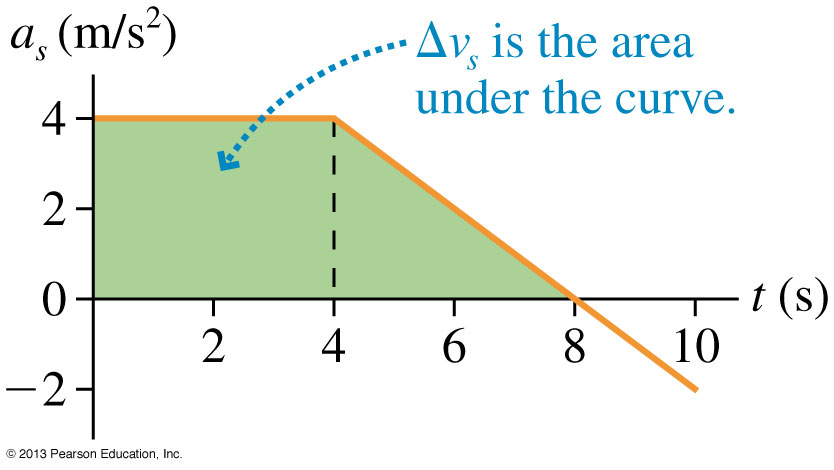
\includegraphics[width=\textwidth]{../figures/02_41_Figure.jpg}
   \uncover<2>{\\$v_s(t=8 \text{ s}) = 34$ m/s}
\end{center}
\end{frame}

\begin{frame}{Picture References}
\tiny
Galileo Galilei on the tower (accessed 4 Sep 17): \href{https://i.pinimg.com/736x/ab/f2/7b/abf27bfdda4a9d19c810ab78964cdff1--galileo-experiment-biology.jpg}{https://i.pinimg.com/736x/ab/f2/7b/abf27bfdda4a9d19c810ab78964cdff1--galileo-experiment-biology.jpg}
\end{frame}

\end{document}
